% ------------------------------------------------------------------------------
% TYPO3 Version 10.0 - What's New (Serbian Version)
%
% @author	Michael Schams <schams.net>
% @license	Creative Commons BY-NC-SA 3.0
% @link		http://typo3.org/download/release-notes/whats-new/
% @language	Serbian
% ------------------------------------------------------------------------------

\section{Izmene za programere}
\begin{frame}[fragile]
	\frametitle{Izmene za programere}

	\begin{center}\huge{Poglavlje 4:}\end{center}
	\begin{center}\huge{\color{typo3darkgrey}\textbf{Izmene za programere}}\end{center}

\end{frame}

% ------------------------------------------------------------------------------
% TYPO3 Version 10.0 - Breaking Changes

% ------------------------------------------------------------------------------
% TYPO3 Version 10.0 - Breaking Changes

\begin{frame}[fragile]
	\frametitle{Izmene za programere}
	\framesubtitle{Korenite izmene - Breaking Changes}

	\small
		Programeri obratite pažnju: u TYPO3 v9, deo PHP koda, TSconfig-a, TypoScript
        opcija i uslova, kao i Scheduler tasks-ova je oznacen kao zastareo.

		\vspace{0.2cm}

		U skladu sa TYPO3 \textbf{poilitikom zastarelost}, ove komponente su izmenjene ili
		uklonjene u TYPO3 v10.0.

		\vspace{0.2cm}

		Ovo takodje ukljucuje neke hook-ove, PHP anotacije (kao na primer \texttt{@inject} i
		\texttt{@validate}), kao i neke izmene vidljivosti (na primer iz
		"\texttt{public}" u "\texttt{protected}").

		\vspace{0.2cm}

		Ukljucite deprecation log, pažljivo testirajte kod i pregledajte log da locirate
		potencijalne probleme. Koristite ugradjeni
		\href{https://docs.typo3.org/m/typo3/reference-coreapi/master/en-us/ApiOverview/ExtensionScanner/Index.html}{Extension Scanner}
		da dobijete ceo izveštaj o proširenjima koja nisu kompatiblilna.

	\normalsize

\end{frame}

% ------------------------------------------------------------------------------
% Feature | 88643 | New Mail API based on symfony/mailer and symfony/mime
% Breaking | 88643 | Removed Swiftmailerswiftmailer Dependency

\begin{frame}[fragile]
	\frametitle{Izmene za programere}
	\framesubtitle{Novi Mail API}

	\begin{itemize}
		\item SwiftMailer je zamenjen modernijim bibliotekama:

			\begin{itemize}
				\item \texttt{symfony/mime} za kreiranje mejl poruka
				\item \texttt{symfony/mailer} za slanje mejlova
			\end{itemize}

		\item PHP funkcija \texttt{mail()} više nije podržana.

			\begin{itemize}\smaller
				\item[\ding{228}] Preporuka je da se prebaci na \texttt{sendmail} ili \texttt{smtp}.
			\end{itemize}\normalsize

		\item Prilagodjeni SwiftMailer plaginovi i transporti zahtevaju migraciju.

		\item Pogledajte \href{https://symfony.com/doc/current/mailer.html}{Symfony Documentation}
			za više detalja kako da iskoristite prednosti novog Mail API-ja.
	\end{itemize}

\end{frame}

% ------------------------------------------------------------------------------
% Feature | 84112 | Symfony dependency injection for core and Extbase

\begin{frame}[fragile]
	\frametitle{Izmene za programere}
	\framesubtitle{Symfony Dependency Management/Injection (1)}

	\begin{itemize}
		\item Paket \texttt{symfony/dependency-injection} je integrisan i koristi se za
			upravljanje zavisnostima i dependency injection-om za klase.

		\item Ovaj pristup ima za cilj da se zameni postojeci Extbase dependency injection
			container i object manager.

		\item Iz tog razloga, sledece klase treba prilagoditi i izbegavati (kad god je moguce):

			\begin{itemize}\small
				\item \texttt{\textbackslash
					TYPO3\textbackslash
					CMS\textbackslash
					Extbase\textbackslash
					Object\textbackslash
					ObjectManager}
				\item \texttt{\textbackslash
					TYPO3\textbackslash
					CMS\textbackslash
					Core\textbackslash
					Utility\textbackslash
					GeneralUtility::makeInstance()}
			\end{itemize}\normalsize

	\end{itemize}

\end{frame}

% ------------------------------------------------------------------------------
% Feature | 84112 | Symfony dependency injection for core and Extbase

\begin{frame}[fragile]
	\frametitle{Izmene za programere}
	\framesubtitle{Symfony Dependency Management/Injection (2)}

	% decrease font size for code listing
	\lstset{basicstyle=\tiny\ttfamily}

	\begin{itemize}
		\item Opcije konfiguracije sadrže:

			\begin{itemize}
				\item Autowiring (pogeldajte sledeci primer)
				\item Manual wiring
					(pogledajte \href{https://docs.typo3.org/c/typo3/cms-core/master/en-us/Changelog/10.0/Feature-84112-SymfonyDependencyInjectionForCoreAndExtbase.html}{change log})
				\item Advanced functionality
					(pogledajte \href{https://docs.typo3.org/c/typo3/cms-core/master/en-us/Changelog/10.0/Feature-84112-SymfonyDependencyInjectionForCoreAndExtbase.html}{change log})
			\end{itemize}

		% \smaller For example "autowiring":\normalsize

\begin{lstlisting}
# Configuration/Services.yaml
services:
  _defaults:
    autowire: true
    autoconfigure: true
    public: false

  Your\Namespace\:
    resource: '../Classes/*'
\end{lstlisting}

		\item Pogledajte \href{https://symfony.com/doc/current/service_container.html}{Symfony documentation} za više detalja.

	\end{itemize}

\end{frame}

% ------------------------------------------------------------------------------
% Feature | 88769 | Introduce a generic EventDispatcher based on PSR-14
% Feature | 88770 | Add PSR-14 EventDispatcher logic based on DI

\begin{frame}[fragile]
	\frametitle{Izmene za programere}
	\framesubtitle{Event Dispatching (1)}

	\begin{itemize}
		\item Novi "EventDispatcher" sistem je dodat i ima za cilj da zameni hook-ove i Signal/Slots koncepte.

		\item Zasnovan je na \href{https://www.php-fig.org/psr/psr-14}{PSR-14 standardu}
			koji omogucava programerima da ubace logiku u aplikaciju lako i konzistentno.

		\item PSR-14 se sastoji od sledece cetiri komponente:

			\begin{itemize}
				\item \textbf{EventDispatcher} objekat koji se koristi da pokrene dogadjaj.
				\item \textbf{ListenerProvider} objekat koji sadrži registrovane Event Listeners-e za sve dogadjaje.
				\item Jedan ili više \textbf{Event} objekata koji se pozivaju iz TYPO3 jezgra ili proširenja ("Emitter").
				\item Jedan ili više \textbf{Listeners-a} (obicno u proširenju i PHP paketima) koji su registrovani.
			\end{itemize}

% Short-Term goal is to deprecate SignalSlot dispatcher in TYPO3 v10,
% and migrate all signals to the EventDispatcher.

	\end{itemize}

\end{frame}

% ------------------------------------------------------------------------------
% Feature | 88769 | Introduce a generic EventDispatcher based on PSR-14
% Feature | 88770 | Add PSR-14 EventDispatcher logic based on DI

\begin{frame}[fragile]
	\frametitle{Izmene za programere}
	\framesubtitle{Event Dispatching (2)}

	% decrease font size for code listing
	\lstset{basicstyle=\tiny\ttfamily}

	Primer implementacije

	\begin{itemize}\smaller
		\item[\ding{202}] Dodajte \texttt{event.listener} tag u fajl \texttt{Configuration/Services.yaml}:

\begin{lstlisting}
services:
  Vendor\Example\EventListener\NullMailer:
    tags:
      - { name: event.listener, identifier: 'myListener', event: TYPO3\CMS\Core\Mail\Event\AfterMailerInitializationEvent, before: 'redirects, anotherIdentifier' }
\end{lstlisting}

		\item[\ding{203}] Implementacija Vašeg objekta dogadjaja:

\begin{lstlisting}
namespace Vendor\Example\EventListener;

class NullMailer
{
  public function __invoke(AfterMailerInitializationEvent $event): void
  {
    $event->getMailer()->injectMailSettings(['transport' => 'null']);
  }
}
\end{lstlisting}

	\end{itemize}\normalsize

\end{frame}

% ------------------------------------------------------------------------------
% Feature | 88769 | Introduce a generic EventDispatcher based on PSR-14
% Feature | 88770 | Add PSR-14 EventDispatcher logic based on DI

\begin{frame}[fragile]
	\frametitle{Izmene za programere}
	\framesubtitle{Event Dispatching (3)}

	% decrease font size for code listing
	\lstset{basicstyle=\tiny\ttfamily}

	\begin{itemize}
		\item Listi dostupnih Event Listeners-a se može pristupiti iz administratorskog interfejsa:\newline
			\smaller
				(zahteva sistemsko proširenje \texttt{EXT:lowlevel})
			\normalsize
	\end{itemize}

	\begin{figure}
		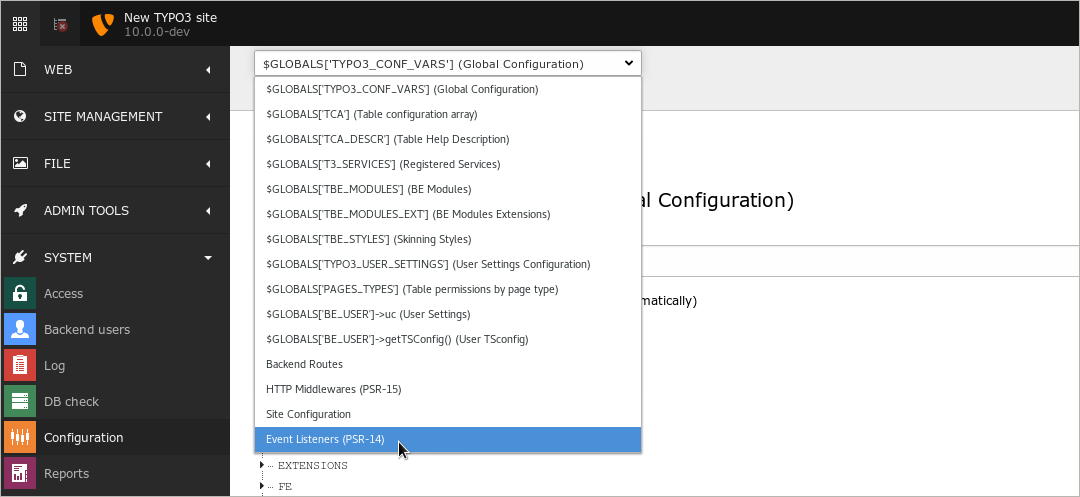
\includegraphics[width=0.70\linewidth]{ChangesForDevelopers/88770-PSR14-EventDispatcher.png}
	\end{figure}

\end{frame}


% ------------------------------------------------------------------------------
% Feature | 88769 | Introduce a generic EventDispatcher based on PSR-14
% Feature | 88770 | Add PSR-14 EventDispatcher logic based on DI

\begin{frame}[fragile]
	\frametitle{Izmene za programere}
	\framesubtitle{Event Dispatching (4)}

	% decrease font size for code listing
	\lstset{basicstyle=\tiny\ttfamily}

	\begin{itemize}
		\item Najbolja praksa:

			\begin{itemize}
				\item Dodajte samo jedan Listener po PHP klasi i koristiti \texttt{\_\_invoke()} kao naziv metode.
				\item Dodajte "\texttt{Event}" sufiks na ime klase kada kreirate novu Event PHP klasu.
				\item Premestite Event PHP klasu u odgovarajuci direktorijum, na primer \texttt{Classes/Database/Event}.
				\item Koristite dependency injection kao argumenat konstruktora da dobijte EventDispatcher objekat, ako je moguce.
			\end{itemize}

		\item Dodatna napomena:\newline
			\small
				Dogadjaji omoguceni od strane TYPO3 jezgra prate TYPO3 politiku zastarevanja, osim za argument konstruktora, koji može da se menja.

			\normalsize

	\end{itemize}

\end{frame}

% ------------------------------------------------------------------------------
% Feature | 88799 | Use PSR-3 interface for logging

\begin{frame}[fragile]
	\frametitle{Izmene za programere}
	\framesubtitle{PSR-3 interfejs za logovanje}

	\begin{itemize}
		\item TYPO3 Logging Framework (u praksi LogLevel i LogManager) sada koriste
			\href{https://www.php-fig.org/psr/psr-3/}{PSR-3 Logger Interface}.

		\item PSR-3 je standardizovan metod koji omogucava da biblioteke prihvataju
			\texttt{Psr\textbackslash
				Log\textbackslash
				LoggerInterface} objekat i da ispisuju logove na jednostavan i univerzalan nacin.

			\item Ovo omogucava programerima da koriste prilagodjene logere i da komuniciraju
				sa drugim sistemima logovanja.

	\end{itemize}

\end{frame}

% ------------------------------------------------------------------------------
% Breaking | 88182 | jsfunc.inline.js has been dropped
% Breaking | 88427 | jsfunc.evalfield.js has been removed
% Breaking | 88667 | Removed additionalJavaScriptSubmit from FormEngine
% Deprecation | 88433 | Deprecate top.openUrlInWindow

\begin{frame}[fragile]
	\frametitle{Izmene za programere}
	\framesubtitle{JavaScript opcije i funkcije (1)}

	\begin{itemize}
		\item Sledeci JavaScript fajlovi su uklonjeni:

			\begin{itemize}
				\item \texttt{jsfunc.inline.js}
				\item \texttt{jsfunc.evalfield.js}
			\end{itemize}

			\begin{itemize}\smaller
				\item[\ding{228}] Umesto njih koristite \texttt{TYPO3/CMS/Backend/FormEngineValidation}.
			\end{itemize}\normalsize

		\item Ranije je bilo moguce dodati dodatne submit handler-e korišcenjem opcije \texttt{additionalJavaScriptSubmit}.
			Ova opcija je uklonjena.

			\begin{itemize}\smaller
				\item[\ding{228}] Umesto toga napravite i registrujte AMD modul.
			\end{itemize}\normalsize

		\item Globalna JavaScript funkcija \texttt{top.openUrlInWindow()} je oznacena kao zastarela.

	\end{itemize}

\end{frame}

% ------------------------------------------------------------------------------
% Breaking | 88411 | TBE_EDITOR.typo3form removed
% Deprecation | 88432 | Replaced md5js with an AMD module
% Deprecation | 88428 | top.rawurlencode and top.str_replace
% Deprecation | 88651 | Replace TYPO3/CMS/Backend/SplitButtons with TYPO3/CMS/Backend/DocumentSaveActions

\begin{frame}[fragile]
	\frametitle{Izmene za programere}
	\framesubtitle{JavaScript opcije i funkcije (2)}

	\begin{itemize}

		\item Globalni objekat \texttt{TBE\_EDITOR.typo3form} i njegovi pomocni šabloni \texttt{typo3FormFieldSet}
			i \texttt{typo3FormFieldGet} su uklonjeni.

		\item Fajl \texttt{md5.js} je oznacen kao zastareo.

			\begin{itemize}\smaller
				\item[\ding{228}] Umesto toga ucitajte AMD modul \texttt{TYPO3/CMS/Backend/Hashing/Md5} korišcenjem RequireJS.
			\end{itemize}\normalsize

		\item Sledece globalne JavaScript funkcije su oznacene kao zastarele:

		\begin{itemize}
			\item \texttt{top.rawurlencode()}
			\item \texttt{top.str\_replace()}
		\end{itemize}

		\item Modul \texttt{TYPO3/CMS/Backend.SplitButtons} je oznacen kao zastareo.

			\begin{itemize}\smaller
				\item[\ding{228}] Umesto njega koristite \texttt{TYPO3/CMS/Backend/DocumentSaveActions}.
			\end{itemize}\normalsize

 	\end{itemize}

\end{frame}

% ------------------------------------------------------------------------------
% Important | 87894 | Removed PHP Dependency algo26-matthiasidna-convert

\begin{frame}[fragile]
	\frametitle{Izmene za programere}
	\framesubtitle{Domeni na UTF-8 osnovi}

	\begin{itemize}
		\item PHP ima funkcije da konvertuje domene iz UTF-8 u IDNA ASCII formu (“punicode”),
			na primer \href{https://www.php.net/manual/en/function.idn-to-ascii.php}{idn\_to\_ascii()}.

		\item Ovo se može koristiti ukoliko je instalirano
			"\href{https://www.php.net/manual/en/book.intl.php}{intl}" PHP proširenje.

		\item Ukoliko PHP proširenje nije instalirano, paket \texttt{symfony/polyfill-intl-idn}
			pruža ovu funkcionalnost.

		\item Prethodno se koristio paket \texttt{algo26-matthias/idna-convert}, medjutim on je sada uklonjen.

	\end{itemize}

\end{frame}

% ------------------------------------------------------------------------------
% Feature | 87665 | Introduce BitSet class

\begin{frame}[fragile]
	\frametitle{Izmene za programere}
	\framesubtitle{BitSet klasa}

	% decrease font size for code listing
	\lstset{basicstyle=\tiny\ttfamily}

	\begin{itemize}
		\item Dodata je nova klasa da efikasno upravlja boolean flag-ovima:\newline
			\texttt{TYPO3\textbackslash
				CMS\textbackslash
				Core\textbackslash
				Type\textbackslash
				BitSet}

		\item Na primer:

\begin{lstlisting}
define('PERMISSIONS_NONE', 0b0); // 0
define('PERMISSIONS_PAGE_SHOW', 0b1); // 1
define('PERMISSIONS_PAGE_EDIT', 0b10); // 2
define('PERMISSIONS_PAGE_DELETE', 0b100); // 4
define('PERMISSIONS_PAGE_NEW', 0b1000); // 8
define('PERMISSIONS_CONTENT_EDIT', 0b10000); // 16
define('PERMISSIONS_ALL', 0b11111); // 31

$bitSet = new \TYPO3\CMS\Core\Type\BitSet(PERMISSIONS_PAGE_SHOW | PERMISSIONS_PAGE_NEW);
$bitSet->get(PERMISSIONS_PAGE_SHOW); // true
$bitSet->get(PERMISSIONS_CONTENT_EDIT); // false
\end{lstlisting}

	\end{itemize}

\end{frame}

% ------------------------------------------------------------------------------
% Important | 87516 | Remove Core HTTP Request Handler Interface

\begin{frame}[fragile]
	\frametitle{Izmene za programere}
	\framesubtitle{Upravljac zahtevima (1)}

	\begin{itemize}
		\item Sledeci interfejs je uklonjen u korist PSR-15 upravljaca zahtevima i middleware interfejsa:\newline
			\texttt{TYPO3\textbackslash
				CMS\textbackslash
				Core\textbackslash
				Http\textbackslash
				RequestHandlerInterface}

	\end{itemize}

\end{frame}

% ------------------------------------------------------------------------------
% Breaking | 88687 | Configure extbase request handlers via PHP

\begin{frame}[fragile]
	\frametitle{Izmene za programere}
	\framesubtitle{Upravljac zahtevima (2)}

	% decrease font size for code listing
	\lstset{basicstyle=\tiny\ttfamily}

	\begin{itemize}
		\item Konfigurisanje Extbase upravljaca zahtevima više nije moguce putemTypoScript-a.

		\smaller\textbf{Stari} metod u TypoScript-u:\normalsize
\begin{lstlisting}
config.tx_extbase {
  mvc {
    requestHandlers {
      Vendor\Example\Mvc\Web\FrontendRequestHandler = Vendor\Example\Mvc\Web\FrontendRequestHandler
    }
  }
}
\end{lstlisting}

		\smaller\textbf{Novi} metod u fajlu \texttt{Configuration/Extbase/RequestHandlers.php}:\normalsize
\begin{lstlisting}
<?php
declare(strict_types = 1);

return [
  \Vendor\Example\Mvc\Web\FrontendRequestHandler::class,
];
\end{lstlisting}

	\end{itemize}

\end{frame}


% ------------------------------------------------------------------------------
% Deprecation | 88366 | Default caching framework cache names changed

\begin{frame}[fragile]
	\frametitle{Izmene za programere}
	\framesubtitle{Caching Framework}

	% decrease font size for code listing
	\lstset{basicstyle=\tiny\ttfamily}

	\begin{itemize}
		\item Sledeci keševi su preimenovani:

			\begin{itemize}\smaller
				\item \texttt{cache\_core} \textrightarrow\hspace{0.1cm}\texttt{core}
				\item \texttt{cache\_hash} \textrightarrow\hspace{0.1cm}\texttt{hash}
				\item \texttt{cache\_pages} \textrightarrow\hspace{0.1cm}\texttt{pages}
				\item \texttt{cache\_pagesection} \textrightarrow\hspace{0.1cm}\texttt{pagesection}
				\item \texttt{cache\_runtime} \textrightarrow\hspace{0.1cm}\texttt{runtime}
				\item \texttt{cache\_rootline} \textrightarrow\hspace{0.1cm}\texttt{rootline}
				\item \texttt{cache\_imagesizes} \textrightarrow\hspace{0.1cm}\texttt{imagesizes}
			\end{itemize}\normalsize

		\item Nova metoda za pristup keševima:

\begin{lstlisting}
STARO:
$cacheManager->getCache('cache_core').

NOVO:
$cacheManager->getCache('core')
\end{lstlisting}

		\item Prefiks \texttt{cf\_} je uklonjen iz imena tabela u bazi podataka.
	\end{itemize}

\end{frame}

% ------------------------------------------------------------------------------
% Deprecation | 87550 | Use controller classes when registering plugins/modules

\begin{frame}[fragile]
	\frametitle{Izmene za programere}
	\framesubtitle{Extbase i Fluid}

	% decrease font size for code listing
	\lstset{basicstyle=\tiny\ttfamily}

	\begin{itemize}
		\item Registrovanje plagina/modula sada zahteva puno ime klase

			\begin{itemize}\smaller
				\item \texttt{\textbackslash
					TYPO3\textbackslash
					CMS\textbackslash
					Extbase\textbackslash
					Utility\textbackslash
					ExtensionUtility::configurePlugin()}
				\item \texttt{\textbackslash
					TYPO3\textbackslash
					CMS\textbackslash
					Extbase\textbackslash
					Utility\textbackslash
					ExtensionUtility::registerModule()}
			\end{itemize}\normalsize

		\item Takodje, izbaciti ime vendora u imenu proširenja (prvi argument).

			\begin{itemize}\smaller
				\item[\ding{228}] Koristiti "\texttt{ExampleBlog}" umesto "\texttt{Vendor.ExampleBlog}".
			\end{itemize}

		\item Na primer:

\begin{lstlisting}
\TYPO3\CMS\Extbase\Utility\ExtensionUtility::configurePlugin(
  'ExampleBlog', // previously: 'Vendor.ExampleBlog'
  'pi1',
  [
    \Vendor\Example\Controller\BlogController::class => 'list,update,delete'
  ],
  [
    \Vendor\Example\Controller\BlogController::class => 'list,update,delete'
  ]
);
\end{lstlisting}

	\end{itemize}

\end{frame}

% ------------------------------------------------------------------------------
% Breaking | 87627 | Remove Property extensionName of AbstractController

\begin{frame}[fragile]
	\frametitle{Deprecated/Removed Functions}
	\framesubtitle{Extbase i Fluid}

	\begin{itemize}
		\item Osobina \texttt{extensionName} iz AbstractController je uklonjena.

			\begin{itemize}\smaller
				\item[\ding{228}] Koristite umesto toga \texttt{\textbackslash
					TYPO3\textbackslash
					CMS\textbackslash
					Extbase\textbackslash
					Mvc\textbackslash
					Request::getControllerExtensionName()}.
			\end{itemize}\normalsize

	\end{itemize}

\end{frame}

% ------------------------------------------------------------------------------
% Feature | 87457 | Use symfony/propertyinfo to gather doc block information

\begin{frame}[fragile]
	\frametitle{Izmene za programere}
	\framesubtitle{Extbase i Fluid}

	% decrease font size for code listing
	\lstset{basicstyle=\tiny\ttfamily}

	\begin{itemize}
		\item Extbase modeli sada podržavaju nepotpuno ime klase u DocBlock-u.

\begin{lstlisting}
use TYPO3\CMS\Extbase\Persistence\ObjectStorage;
use ExtbaseTeam\BlogExample\Domain\Model\Comment;

class Post
{
  /**
   * @var ObjectStorage<Comment>
   */
  public $comments;
}
\end{lstlisting}

	\end{itemize}

\end{frame}

% ------------------------------------------------------------------------------
% Breaking | 87957 | Validators are not registered automatically in Extbase anymore

\begin{frame}[fragile]
	\frametitle{Izmene za programere}
	\framesubtitle{Extbase i Fluid}

	% decrease font size for code listing
	\lstset{basicstyle=\tiny\ttfamily}

	\begin{itemize}
		\item Validatori više nisu automatski registrovani u Extbase.
		\item Za model pod nazivom
			\small\texttt{Vendor\textbackslash
				Example\textbackslash
				Domain\textbackslash
				Model\textbackslash
				Blog}\normalsize,\newline
			Extbase je automatski koristio validator
			\small\texttt{Vendor\textbackslash
				Example\textbackslash
				Domain\textbackslash
				Validator\textbackslash
				BlogValidator}\normalsize

		\item Validatori sada moraju biti rucno registrovani:

\begin{lstlisting}
use Vendor\Example\Domain\Model\Blog;
use TYPO3\CMS\Extbase\Annotation as Extbase;
use TYPO3\CMS\Extbase\Mvc\Controller\ActionController;

class BlogController extends ActionController
{
  /**
   * @Extbase\Validate(param="blog", validator="Vendor\Example\Domain\Validator\BlogValidator")
   */
  public function showAction(Blog $blog)
  {
    // ...
  }
}
\end{lstlisting}

	\end{itemize}

\end{frame}

% ------------------------------------------------------------------------------
% Breaking | 87623 | Replace config.persistence.classes typoscript configuration (1)

\begin{frame}[fragile]
	\frametitle{Izmene za programere}
	\framesubtitle{Extbase i Fluid - mapiranje klasa (1)}

	% decrease font size for code listing
	\lstset{basicstyle=\tiny\ttfamily}

	\begin{itemize}
		\item Mapiranje klasa vezanih za persistence korišcenjem TypoScript-a više nije moguce:

\begin{lstlisting}
config.tx_example_blog {
  persistence {
    classes {
      Vendor\Example\Domain\Model\Author {
        mapping {
          tableName = fe_users
          columns.name.mapOnProperty = fullname
        }
      }
    }
  }
}
\end{lstlisting}

	\end{itemize}

\end{frame}

% ------------------------------------------------------------------------------
% Breaking | 87623 | Replace config.persistence.classes typoscript configuration (2)

\begin{frame}[fragile]
	\frametitle{Izmene za programere}
	\framesubtitle{Extbase i Fluid - mapiranje klasa (2)}

	% decrease font size for code listing
	\lstset{basicstyle=\tiny\ttfamily}

	\begin{itemize}
		\item Mapiranje se mora izvršiti u PHP fajlu \texttt{Configuration/Extbase/Persistence/Classes.php}:

\begin{lstlisting}
<?php
declare(strict_types = 1);

return [
  \Vendor\Example\Domain\Model\Author::class => [
    'tableName' => 'fe_users',
    'properties' => [
      'name' => [
        'fieldName' => 'fullname'
      ]
    ]
  ]
];
\end{lstlisting}

	\end{itemize}

\end{frame}

% ------------------------------------------------------------------------------
% Breaking | 87594 | Harden Extbase

\begin{frame}[fragile]
	\frametitle{Izmene za programere}
	\framesubtitle{Extbase i Fluid}

	% decrease font size for code listing
	\lstset{basicstyle=\smaller\ttfamily}

	\begin{itemize}
		\item Klase sada poseduju "strict type" mod i type hints za skalarne promenljive

\begin{lstlisting}
<?php
declare(strict_types=1);
\end{lstlisting}

		% Method signatures in Extbase classes have been updated.
		\item Ovo izaziva PHP fatal errors ukoliko potpis metode u prilagodjenom
			proširenju nije u skladu sa interfejsom i/ili parent klasom.


		\item Pogledajte \href{https://forge.typo3.org/issues/87594}{forge \#87594}
			za kompletnu listu svih promena.

		\item Ovaj zadatak je i dalje u toku i moguce su dodatne promene.

	\end{itemize}

\end{frame}

% ------------------------------------------------------------------------------
% Breaking | 87937 | TCA option selicon_field_path removed
% Breaking | 87989 | TCA option setToDefaultOnCopy removed
% Breaking | 87936 | TCA for sys_history removed

\begin{frame}[fragile]
	\frametitle{Izmene za programere}
	\framesubtitle{TCA izmene}

	\begin{itemize}
		\item Sledece TCA opcije su uklonjene:

			\begin{itemize}
				\item \texttt{\$TCA[\$tableName]['ctrl']['selicon\_field\_path']}
				\item \texttt{\$TCA[\$tableName]['ctrl']['setToDefaultOnCopy']}
			\end{itemize}

			\begin{itemize}\smaller
				\item[\ding{228}] Kada se kopiraju rekordi, DataHandler treba da se koristi da se polja resetuju.
			\end{itemize}\normalsize

		\item Kompletan TCA od \texttt{sys\_history} je uklonjen i polje u bazi podataka \texttt{pid} je takodje uklonjeno.
			Pristup \texttt{\$GLOBALS['TCA']['sys\_history']} izaziva PHP warning.

	\end{itemize}

\end{frame}

% ------------------------------------------------------------------------------
% Breaking | 88527 | Overriding custom values in User Authentication derivatives

\begin{frame}[fragile]
	\frametitle{Izmene za programere}
	\framesubtitle{Autentikacija korisnika klase/servisi (1)}

	\begin{itemize}
		\item Restruktuirana je sledeca apstraktna klasa:\newline
			\small\texttt{TYPO3\textbackslash
				CMS\textbackslash
				Core\textbackslash
				Authentication\textbackslash
				AbstractUserAuthentication}\normalsize
		\item Ovo takodje ukljucuje i dve direktne pod-klase:

			\begin{itemize}
				\item \texttt{BackendUserAuthentication}
				\item \texttt{FrontendUserAuthentication}
			\end{itemize}

		\item Izmena utice na osobine:

			\begin{itemize}
				\item \texttt{sessionTimeout}
				\item \texttt{gc\_time}
				\item \texttt{sessionDataLifetime}
				\item \texttt{loginType}
			\end{itemize}

	\end{itemize}

\end{frame}

% ------------------------------------------------------------------------------
% Breaking | 88646 | Removed inheritance of AbstractService from AbstractAuthenticationService

\begin{frame}[fragile]
	\frametitle{Izmene za programere}
	\framesubtitle{Autentikacija korisnika klase/servisi (2)}

	\begin{itemize}

		\item Sledeca klasa više ne nasledjuje
			\smaller\texttt{AbstractService}\normalsize\hspace{0.1cm}:
			\smaller\texttt{\textbackslash
				TYPO3\textbackslash
				CMS\textbackslash
				Core\textbackslash
				Authentication\textbackslash
				AbstractAuthenticationService}\normalsize

		\item Ovo može da utice na neke hook-ove i prilagodjene provajdere za autentikaciju.

		\item Programerima se savetuje da pregledaju prilagodjene servise za autentikaciju i ažuriraju kod ako je neophodno.


	\end{itemize}

\end{frame}

% ------------------------------------------------------------------------------
% Deprecation | 87882 | File related controllers moved to EXT:filelist

\begin{frame}[fragile]
	\frametitle{Izmene za programere}
	\framesubtitle{Kontorleri liste fajlova (Filelist)}

	\begin{itemize}
		\item Sledeci kontorleri su premešteni u \texttt{EXT:filelist}:

			\begin{itemize}\small
				\item \texttt{CreateFolderController}
				\item \texttt{EditFileController}
				\item \texttt{FileUploadController}
				\item \texttt{RenameFileController}
				\item \texttt{ReplaceFileController}
			\end{itemize}\normalsize

		\item Kao rezultat toga, namespace je takodje promenjen:\newline
			\texttt{\textbackslash
				TYPO3\textbackslash
				CMS\textbackslash
				Filelist\textbackslash
				Controller\textbackslash
				File}

		\vspace{0.2cm}

		\small
			Napomena: Koristite TYPO3 FAL kao API i dodajte svoje funkcionalnosti
			sa Vašim kontorlerima, umesto da koristite \textbf{postojece}
			kontrolere izlistane gore.
		\normalsize

	\end{itemize}

\end{frame}

% ------------------------------------------------------------------------------
% Deprecation | 88499 | BackendUtility::getViewDomain()

\begin{frame}[fragile]
	\frametitle{Izmene za programere}
	\framesubtitle{URL za prikaz korisnickog interfejsa}

	% decrease font size for code listing
	\lstset{basicstyle=\tiny\ttfamily}

	\begin{itemize}
		\item Sledeca staticka metoda je oznacena kao zastarela:\newline
			\smaller\texttt{\textbackslash
				TYPO3\textbackslash
				CMS\textbackslash
				Backend\textbackslash
				Utility\textbackslash
				BackendUtility::getViewDomain()}\normalsize

		\item Zamenite metodu direktnim detektovanjem sajta na osnovu ID-ja stranice u TYPO3 administratorskom interfejsu.
		\item Na primer:

\begin{lstlisting}
$pageId = 123;
$site = GeneralUtility::makeInstance(SiteFinder::class)->getSiteByPageId($pageId);
$url = $site->getRouter()->generateUri($pageId, ['type' => 13]);
\end{lstlisting}

	\end{itemize}

\end{frame}

% ------------------------------------------------------------------------------
% Deprecation | 88406 | setCacheHash/noCacheHash options in ViewHelpers and UriBuilder

\begin{frame}[fragile]
	\frametitle{Izmene za programere}
	\framesubtitle{cHash u UriBuilder-u i ViewHelper-ima}

	% decrease font size for code listing
	\lstset{basicstyle=\smaller\ttfamily}

	\begin{itemize}
		\item Sledece dve Extbase UriBuilder metode su oznacene kao zastarele:

			\begin{itemize}
				\item \texttt{UriBuilder->setUseCacheHash()}
				\item \texttt{UriBuilder->getUseCacheHash()}
			\end{itemize}

		\item Ovo takodje utice na odredjen broj Fluid ViewHelper-a:
	\end{itemize}
	\vspace{-0.4cm}
	\begin{columns}[T]
		\begin{column}{.05\textwidth}
		\end{column}
		\begin{column}{.45\textwidth}
			\begin{itemize}\smaller
				\item \texttt{f:form}
				\item \texttt{f:link.action}
				\item \texttt{f:link.page}
				\item \texttt{f:link.typolink}
				\item \texttt{f:uri.action}
			\end{itemize}\normalsize
		\end{column}
		\begin{column}{.45\textwidth}
			\begin{itemize}\smaller
				\item \texttt{f:uri.page}
				\item \texttt{f:uri.typolink}
				\item \texttt{f:widget.link}
				\item \texttt{f:widget.uri}
			\end{itemize}\normalsize
		\end{column}
	\end{columns}
	\vspace{0.2cm}
	\begin{itemize}
		\item ...kao i na TypoLink opciju "\texttt{useCacheHash}".
	\end{itemize}

\end{frame}

% ------------------------------------------------------------------------------
% Breaking | 88540 | Changed Request Workflow for Frontend Requests

\begin{frame}[fragile]
	\frametitle{Izmene za programere}
	\framesubtitle{Tok zahteva na korisnickom interfejsu}

	% decrease font size for code listing
	\lstset{basicstyle=\smaller\ttfamily}

	\begin{itemize}
		\item Tok zahteva na korisnickom interfejsu je znacajno preuredjen.

		\item Sve komponente koje se koriste su napravljene korišcenjem PSR-15 middleware-a, PSR-15 upravljac zahtevima
			i globalni TypoScriptFrontendController (TSFE) od verzije TYPO3 v9.

		\item Ovo utice na prilagodjeni kod, ukoliko je korišcen sledeci hook i sesija korisnickog interfejsa:\newline
			{\fontsize{7}{8}\selectfont\texttt{\$GLOBALS['TYPO3\_CONF\_VARS']['SC\_OPTIONS']['tslib/class.tslib\_fe.php']['hook\_eofe']}}

			\begin{itemize}\smaller
				\item[\ding{228}] Koristite umesto ovoga PSR-15 middleware, ili direktno pozovite \texttt{storeSessionData}
				u hook-u u PHP-u.
			\end{itemize}\normalsize

	\end{itemize}

\end{frame}

% ------------------------------------------------------------------------------
% Breaking | 88498 | Global data for TimeTracker statistics removed

\begin{frame}[fragile]
	\frametitle{Izmene za programere}
	\framesubtitle{Tok zahteva na korisnickom interfejsu}

	% decrease font size for code listing
	\lstset{basicstyle=\smaller\ttfamily}

	\begin{itemize}
		\item Sledece globalne promenljive su uklonjene:

			\begin{itemize}
				\item \texttt{\$GLOBALS['TYPO3\_MISC']['microtime\_start']}
				\item \texttt{\$GLOBALS['TYPO3\_MISC']['microtime\_end']}
				\item \texttt{\$GLOBALS['TYPO3\_MISC']['microtime\_BE\_USER\_start']}
				\item \texttt{\$GLOBALS['TYPO3\_MISC']['microtime\_BE\_USER\_end']}
			\end{itemize}

		\item TYPO3 jezgro ih je koristilo u Admin Panel-u i HTTP header-u na primer.

			\begin{itemize}\smaller
				\item[\ding{228}] Umesto toga koristite \texttt{TimeTracker->finish()}.
			\end{itemize}\normalsize

	\end{itemize}

\end{frame}


% ------------------------------------------------------------------------------
% Deprecation | 88569 | Locales::initialize() in favor of regular singleton instance
% Deprecation | 88473 | TypoScriptFrontendController->settingLocale

\begin{frame}[fragile]
	\frametitle{Deprecated/Removed Functions}
	\framesubtitle{Locales}

	\begin{itemize}
		\item Metoda \texttt{Locales::initialize()} je oznacena kao zastarela.

			\begin{itemize}\smaller
				\item[\ding{228}] Umesto toga koristite \texttt{GeneralUtility::makeInstance(Locales::class)} ili
				dependency injection da dohvatite instancu klase \texttt{Locales}.
			\end{itemize}\normalsize

		\item Funkcionalnost sledece metode je oznacena kao zastarela:\newline
			\texttt{TypoScriptFrontendController->settingLocale()}.

			\begin{itemize}\smaller
				\item[\ding{228}] Funkcija je sada dostupna kao
				{\fontsize{8}{8} \selectfont \texttt{Locales::setSystemLocaleFromSiteLanguage()}.}
			\end{itemize}\normalsize

	\end{itemize}

\end{frame}

% ------------------------------------------------------------------------------
% Deprecation | 88559 | TSFE->sys_language_isocode

\begin{frame}[fragile]
	\frametitle{Deprecated/Removed Functions}
	\framesubtitle{Locales}

	\begin{itemize}
		\item Javna osobina \texttt{TypoScriptFrontendController->sys\_language\_isocode}
			je oznacena kao zastarela.

			\begin{itemize}\smaller
				\item[\ding{228}] Osobini možete pristupiti putem \texttt{SiteLanguage->getTwoLetterIsoCode()}
				i \texttt{sitelanguage:twoLetterIsoCode}.
			\end{itemize}\normalsize

	\end{itemize}

\end{frame}

% ------------------------------------------------------------------------------
% Breaking | 88458 | Removed Frontend Track User ftu functionality

\begin{frame}[fragile]
	\frametitle{Deprecated/Removed Functions}
	\framesubtitle{Pracenje korisnika na korisnickom interfejsu}

	\begin{itemize}

		\item Uklonjene su sledece javne osobine klase\newline
			\smaller\texttt{\textbackslash
				TYPO3\textbackslash
				CMS\textbackslash
				Core\textbackslash
				Authentication\textbackslash
				AbstractUserAuthentication}:
			\normalsize\newline


			\begin{itemize}\smaller
				\item \texttt{AbstractUserAuthentication->get\_name}
				\item \texttt{AbstractUserAuthentication->getFallBack}
				\item \texttt{AbstractUserAuthentication->getMethodEnabled}
				\item \texttt{AbstractUserAuthentication->get\_URL\_ID}
			\end{itemize}\normalsize

		\item Takodje i osobina \texttt{getMethodUrlIdToken} iz klase\newline
			\smaller\texttt{\textbackslash
				TYPO3\textbackslash
				CMS\textbackslash
				Frontend\textbackslash
				Controller\textbackslash
				TypoScriptFrontendController}.
			\normalsize

		\item Kao i TypoScript podešavanje \texttt{config.ftu},
			kao i globalno podešavanje
			{\fontsize{8}{8} \selectfont \texttt{\$GLOBALS['TYPO3\_CONF\_VARS']['FE']['get\_url\_id\_token']}.}

	\end{itemize}

\end{frame}

% ------------------------------------------------------------------------------
% Breaking | 87305 | Use constructor injection in DataMapper

\begin{frame}[fragile]
	\frametitle{Deprecated/Removed Functions}
	\framesubtitle{Constructor Injection u DataMapper-u}

	\begin{itemize}

		\item Sledeca klasa sada koristi constructor injection umesto setter injection:
			\smaller
				\texttt{\textbackslash
					TYPO3\textbackslash
					CMS\textbackslash
					Extbase\textbackslash
					Persistence\textbackslash
					Generic\textbackslash
					Mapper\textbackslash
					DataMapper}
			\normalsize

			\begin{itemize}\smaller
				\item[\ding{228}] Izbegavajte \texttt{GeneralUtility::makeInstance()} i \texttt{ObjectManager->get()}.
				\item[\ding{228}] Umesto toga koristite dependency injection (preporucljivo constructor injection).
			\end{itemize}\normalsize

	\end{itemize}

\end{frame}

% ------------------------------------------------------------------------------
% Feature | 88791 | Introduce PreviewAspect in Context

\begin{frame}[fragile]
	\frametitle{Deprecated/Removed Functions}
	\framesubtitle{Context API}

	% decrease font size for code listing
	\lstset{basicstyle=\tiny\ttfamily}

	\begin{itemize}

		\item Context API poseduje novi aspekt "\texttt{frontend.preview}"
			koji može da pokaže da li je korisnicki interfejs u "preview" modu:

\begin{lstlisting}
GeneralUtility::makeInstance(Context::class)
  ->getPropertyFromAspect('frontend.preview', 'isPreview');
\end{lstlisting}

		\item Ovaj aspekt menja sledecu osobinu, koja je sada oznacena kao zastarela:
			\small\texttt{TypoScriptFrontendController->fePreview}\normalsize

	\end{itemize}

\end{frame}

% ------------------------------------------------------------------------------
% Feature | 88792 | Add TypoScriptAspect to handle TypoScript Rendering Context settings
% Deprecation | 88792 | forceTemplateParsing in TSFE and TemplateService has been deprecated

\begin{frame}[fragile]
	\frametitle{Deprecated/Removed Functions}
	\framesubtitle{Context API}

	% decrease font size for code listing
	\lstset{basicstyle=\tiny\ttfamily}

	\begin{itemize}

		\item Još jedan novi aspekt \texttt{TypoScriptAspect} može da se koristi da se manipuliše/proveri
			da li je forsiran TemplateRendering.

		\item Podešavanje \texttt{forceTemplateParsing} (TSFE i TemplateService) je oznaceno kao zastarelo.
			Umesto toga treba koristiti Context API:

\begin{lstlisting}
GeneralUtility::makeInstance(Context::class)
  ->getPropertyFromAspect('typoscript', 'forcedTemplateParsing');

$context->setAspect(
  'typoscript',
  GeneralUtility::makeInstance(TypoScriptAspect::class, true)
);
\end{lstlisting}

	\end{itemize}

\end{frame}

% ------------------------------------------------------------------------------
% Breaking | 88525 | Remove “createDirs” directive of extension installation / ext_emconf.php
% Breaking | 87511 | Remove $viewFormatToObjectNameMap property
% Breaking | 87511 | Remove $namespacesViewObjectNamePattern property
% Feature | 87726 | Extend Frontend Login Controller Hook To Validate Password

\begin{frame}[fragile]
	\frametitle{Izmene za programere}
	\framesubtitle{Razno}

	\begin{itemize}
		\item Više nije podržana direktiva \texttt{createDirs} u fajlu \texttt{ext\_emconf.php}.

			\begin{itemize}\smaller
				\item[\ding{228}] Direktorijumi nece biti automatski kreirani prilikom instaliranja proširenja.
			\end{itemize}\normalsize

		\item Uklonjene su sledece dve osobine iz klase
			\texttt{TYPO3\textbackslash
				CMS\textbackslash
				Extbase\textbackslash
				Mvc\textbackslash
				Controller\textbackslash
				ActionController}:\newline

			\begin{itemize}
				\item \texttt{\$namespacesViewObjectNamePattern}
				\item \texttt{\$viewFormatToObjectNameMap}
			\end{itemize}

		\item Sledeci postojeci hook je proširen i sada se može koristiti da validira lozinke:\newline
			{\fontsize{8}{10} \selectfont \texttt{\$GLOBALS['TYPO3\_CONF\_VARS']['EXTCONF']['felogin']['password\_changed']}}

	\end{itemize}

\end{frame}

% ------------------------------------------------------------------------------
% Deprecation | 87613 | Deprecate /TYPO3/CMS/Extbase/Utility/TypeHandlingUtility::hex2bin
% Deprecation | 88554 | Deprecated methods in VersionNumberUtility

\begin{frame}[fragile]
	\frametitle{Izmene za programere}
	\framesubtitle{Razno}

	\begin{itemize}

		\item Sledece metode su oznacene kao zastarele:\newline
			\smaller\texttt{\textbackslash
				TYPO3\textbackslash
				CMS\textbackslash
				Extbase\textbackslash
				Utility\textbackslash
				TypeHandlingUtility::hex2bin()}\normalsize

			\begin{itemize}\smaller
				\item[\ding{228}] Umesto toga koristitie PHP funkciju \href{https://www.php.net/manual/en/function.hex2bin.php}{hex2bin()}.
			\end{itemize}\normalsize

		\item Sledece metode klase
			\smaller\texttt{\textbackslash
				TYPO3\textbackslash
				CMS\textbackslash
				Core\textbackslash
				Utility\textbackslash
				VersionNumberUtility}\normalsize\newline
			su oznacene kao zastarele:

			\begin{itemize}
				\item \texttt{convertIntegerToVersionNumber()}
				\item \texttt{splitVersionRange()}
				\item \texttt{raiseVersionNumber()}
			\end{itemize}

			\begin{itemize}\smaller
				\item[\ding{228}] Implementirajte metode kao prilagodjen kod.
			\end{itemize}\normalsize

	\end{itemize}

\end{frame}

% ------------------------------------------------------------------------------
% Feature | 86964 | Allow getting class property default value
% Deprecation | 82669 | Streamline Backend route path inconsistencies

\begin{frame}[fragile]
	\frametitle{Izmene za programere}
	\framesubtitle{Razno}

	% decrease font size for code listing
	\lstset{basicstyle=\tiny\ttfamily}

	\begin{itemize}
		\item Sada je moguce, korišcenjem ReflectionService-a, dobiti podrazumevanu vrednost
			osobine klase.


\begin{lstlisting}
$property = GeneralUtility::makeInstance(ReflectionService::class)
  ->getClassSchema(MyClass::class)
  ->getProperty('myProperty');
\end{lstlisting}

		\item Rute administratorskog interfejsa, po podrazumevanim podešavanjima, ka modulima bez konfiguracije putanje su sada nazvane\newline
			"\texttt{/module/<main-module>/<sub-module>}"\newline
			\small
				(na primer: "\texttt{/module/web/ts}".)
			\normalsize

		\item Stare rute još uvek funkcionišu (na primer "\texttt{/web/ts/}"), ali ova sintaksa ce biti uklonjena u TYPO3 v11.

	\end{itemize}

\end{frame}

% ------------------------------------------------------------------------------
% Breaking | 88669 | FormEngine FormDataProvider parentPageTca removed
% Breaking | 88744 | Database fields related to CSS Styled Content removed
% Breaking | 88143 | Version-related database field “t3ver_id” removed
% Deprecation | 88746 | PageRepository PHP class moved from Frontend to Core Extension

\begin{frame}[fragile]
	\frametitle{Izmene za programere}
	\framesubtitle{Razno}

	\begin{itemize}
		\item FormEngine DataProvider \texttt{parentPageTca} je uklonjen.

			\begin{itemize}\smaller
				\item[\ding{228}] Programeri mogu direktno da pristupe \texttt{\$GLOBALS['TCA']['pages']}, umesto \texttt{\$result['parentPageTca']}.
			\end{itemize}\normalsize

		\item Sledeca polja u bazi podataka su uklonjena:

			\begin{itemize}\smaller
				\item \texttt{tt\_content.spaceBefore} (zamenjeno poljem \texttt{space\_before\_class})
				\item \texttt{tt\_content.spaceAfter} (zamenjeno poljem \texttt{space\_after\_class})
				\item \texttt{pages.t3ver\_id} (ne koristi se od TYPO3 v9)
			\end{itemize}\normalsize

		\item PHP klasa
			\texttt{\textbackslash
				TYPO3\textbackslash
				CMS\textbackslash
				Frontend\textbackslash
				Page\textbackslash
				PageRepository} je premeštena iz sistemskog proširenja "frontend" u jezgro TYPO3.

			\begin{itemize}\smaller
				\item Zamenite sa klasom:
					\texttt{\textbackslash
						TYPO3\textbackslash
						CMS\textbackslash
						Core\textbackslash
						Domain\textbackslash
						Repository\textbackslash
						PageRepository}
			\end{itemize}\normalsize

	\end{itemize}

\end{frame}

% ------------------------------------------------------------------------------
% Breaking | 88574 | 4th parameter of PageRepository>enableFields removed
% Deprecation | 85895 | Deprecate File::_getMetaData()
% Deprecation | 88662 | Deprecated backend route xMOD_tximpexp

\begin{frame}[fragile]
	\frametitle{Deprecated/Removed Functions}
	\framesubtitle{Razno}

	\begin{itemize}

		\item Cetvrti parametar metode \texttt{PageRepository->enableFields()} je uklonjen.

		\begin{itemize}\smaller
			\item[\ding{228}] Ukoliko programer koristi cetvrti parametar u ovoj metodi, a on je podešen na vrednost "\textbf{false}", ovo može bezbedno da se ukloni.
			\item[\ding{228}] Ukoliko je vrednost podešena na "\textbf{true}", kod mora da se zameni sa posebnom instancom klase \texttt{PageRepository} sa prilagodjenim \texttt{Context-om}.
		\end{itemize}\normalsize

		\item Metoda \texttt{File::\_getMetaData()},  koja se koristila da dohvati meta podatke fajla je oznacena kao zastarela.


			\begin{itemize}\smaller
				\item[\ding{228}] Umesto toga, da dohvatite meta podatke koristite \texttt{\$fileObject->getMetaData()->get()}.
			\end{itemize}\normalsize

		\item Route identifier "\texttt{xMOD\_tximpexp}" je oznacen kao zastareo.

			\begin{itemize}\smaller
				\item[\ding{228}] U zavisnosti od slucaja koristite \texttt{tx\_impexp\_export} ili \texttt{tx\_impexp\_import}.
			\end{itemize}\normalsize

	\end{itemize}

\end{frame}

% ------------------------------------------------------------------------------
% Breaking | 88496 | Method getSwitchableControllerActions has been removed
% Breaking | 87567 | Global variable $TBE_TEMPLATE removed
% Breaking | 88660 | $GLOBALS[T3_VAR] removed

\begin{frame}[fragile]
	\frametitle{Deprecated/Removed Functions}
	\framesubtitle{Razno}

	\begin{itemize}

		\item Sledeca apstraktna metoda je uklonjena:\newline
			\smaller
				\texttt{\textbackslash
					TYPO3\textbackslash
					CMS\textbackslash
					Extbase\textbackslash
					Configuration\textbackslash
					AbstractConfigurationManager::}\newline
					\texttt{getSwitchableControllerActions()}
			\normalsize

			\begin{itemize}\smaller
				\item[\ding{228}] Umesto nje koristite novu metodu \texttt{getControllerConfiguration()} (ista PHP klasa).
			\end{itemize}\normalsize

		\item Globalna promenljiva \texttt{\$TBE\_TEMPLATE} je uklonjena, ukljucujuci
		 	povezani PSR-15 middleware (koji je oznacen kao unutrašnji).

			\begin{itemize}\smaller
				\item[\ding{228}] Instancirajte DocumentTemplate klasu direktno u kontroleru modula.
				\item[\ding{228}] Migirirajte na ModuleTemplate koji je dostupan od TYPO3 v7.
			\end{itemize}\normalsize

		\item Globalna promenljiva \texttt{\$GLOBALS['T3\_VAR']} je uklonjena.\newline

	\end{itemize}

\end{frame}

% ------------------------------------------------------------------------------
